% !TEX encoding = UTF-8
% !TEX TS-program = pdflatex
% !TEX root = ../Tesi.tex
% !TEX spellcheck = it-IT

%************************************************

%************************************************


Designing conversational user interface experience is complicated because conversation comes with many expectations. When these expectations are met, we feel the interface is natural, but once violated, we feel something is amiss. It is important to discuss features that have to be considered in CUI design for specific domain. 

Chatbots are expected to be the new generation of digital product design, after the evolution from Web to mobile applications. The reason lies behind the simplicity offered by the CUI when performing a task, which otherwise could be tedious or requires more time and effort if performed via web or mobile apps. In addition, users spend more time on their messaging platforms than any mobile apps, this generates a new shift to address user needs.

It takes around 18 clicks to perform an airline reservation, while we’re faced with an unwieldy array of buttons, ads, drop-downs, text boxes and more. Simplicity is crucial when communicating with our device. Rather than pulling up an app to search for restaurant, tap to select time and type in number of people, we can simply tell a chatbot to “Book me a table for three at 6 tonight, at the Elzar’s place” \cite{zakos2008}.

Using a chatbot to access a service wont requires users to familiarise themselves with the bot as it is the case with mobile apps.

Although this new paradigm shift, the current state of conversational interface is limited in terms of established user interface design patterns. The current resources on CUI design and the specific bot behaviour in certain domain is limited.

\begin{figure}[htb]
	\centering
	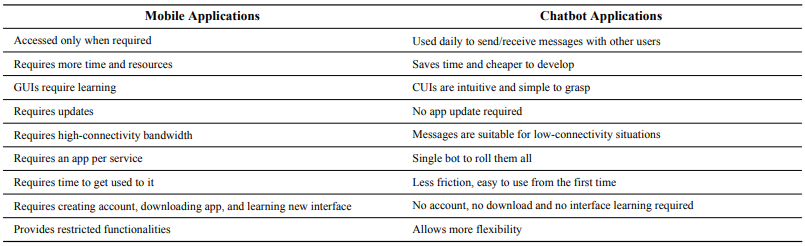
\includegraphics[width = 130mm]{mobile-vs-cui}
	\caption{Major Advantages Of Conversational Interfaces Over Mobile Applications \cite{fadhil2018}.}
	\label{mobile-vs-cui}
\end{figure}


\section{Finance-specific UX Design Patterns}
Domain-specific design patterns can be treated as higher level patterns that can be achieved by using a subset of the methods described in chapter \ref{cap:capitolo2}. 

\subsection{Follow-up questions}
Bots have to ask a set of domain specific questions. These questions depend on situational context in the domain. The number of follow-up questions have to be fixed for a well-defined context. For instance, if the customer has an issue with financial account, then the bot has to provide follow up questions to comprehend if the account is for saving or trading, it is setup for day trading or regular trading, and so on. Therefore, the bot has to reflect the specific domain it is employing by its personality, and it shouldn’t place users in a situation where they need to guess the correct answer. Can be achieved by Flexibility in Response, Conversation Flow, Simplicity in Interaction, Tasks and Duty Specification \cite{fadhil2018}.

\subsection{Cognitive load}
Chatbots can reduce cognitive load and provide emotional link through the conversation. To reduce the cognitive load for users approaches, such as images, buttons, or structured inputs could be used. The bot have to provide clear choices, such as “Black or White” to provide clear indication on how to input information. To achieve a cognitive load in a bot, custom soft keyboards could permit a limited range of inputs and can save a bunch of typing. For example, rather than asking users to type a “Yes” or “No” text, the bot could present two mutually exclusive buttons. Moreover, introducing simplicity and avoiding complicated branching paths could decrease cognitive load. Can be achieved by Text vs Custom Buttons, Simplicity in Interaction, Keep Conversation Short \cite{fadhil2018}.


\subsection{Input validation}
To have an idea of user input, we need to know what is the conversation nature. Therefore, to validate user input we must consider the conversation medium (e.g., text, button, or graphics). Moreover, which technique the bot uses to process the message (e.g., role based, NLP, or some machine learning based). Therefore, we have to consider using text vs custom keyboard, and rigid or NLP syntax when working with CUI input validation. Can be achieved by Text vs Custom Buttons, Tasks and Duty Specification \cite{fadhil2018}.

\subsection{Personalisation} 
In \cite{duijst2017} personalisation is taken into account. The main research question is “What is the added value of personalisation for the user experience of chatbots?”. Two kinds of chatbots have been designed, one with and one without personalisation factors. The design of this research is a two-by-two factorial design. The independent variables are the two chatbots (unpersonalised versus personalised) and the specific task or goal the user can achieve with the chatbot in the financial field (a simple versus a complex task). The results are that there was no significant interaction effect between personalisation and task on the user experience of chatbots. 

\section{Some analysis}
% Some results

\subsubsection{Voice vs text}
In \cite{kim2018} a study was conducted to analyze differences in human-chatbot interactions based on input modality.

Altough giving spoken orders was more convenient and helpful than written orders, users worried that the voice recognition might not work, so they delivered their speech syllable by syllable to articulate their commands. Voice-input modality subjects tended to explain themselves in detail and at great length. This kind of behavior was likely based on the belief that the banking chatbot could understand human speech as a form of communication. But the main concern was about saying things out loud to the chatbot in public. In addition, users were concerned about misunderstandings and errors occurred during transactions.


\subsubsection{Feeling safe}
A sense of insecurity is one of the reasons consumers do not already interact with financial institutions on social media\cite{letheren2017}. The trade-off between the convenience and security of a service comes down to trust. Trust in the service provider to protect our personal details (“soft trust”) and trust in the platform and infrastructure you use to access the service (“hard trust”). Both types of trust are important to ensure a sense of balance. Banks previously used physical design to create a sense of security and trust. This is called signalling and involved the use of marble floors, metal bars, and imposing vaults in bank branches to reassure us that our money is safe. As banking shifted into apps and websites, banks faced the same problem as chatbots currently do,the internet was undoubtedly more convenient but at the expense of a feeling of safety. This was also solved with design. Websites and apps were designed to send similar signals as that of the physical bank branches. For instance, by logging customers out if they’re inactive for too long, and moving keyboards for entering online banking passwords. Consumers feel more secure when a system generates a unique password for each login, than they do when they are allowed a permanent password. Even seeing the initials of an employee in a Tweet can humanise the interaction and instil trust. All of these design aspects evolved to signal trust and security. But chatbots do not have access to these same design capabilities. On the back end, chatbots can be secured just like websites and appsbut it’s important to promote this feeling in users too. A big part of it will be “humanizing” the interaction. For instance, chatbots can be programmed to seem more human, achieving the same thing as staff members’ initials on social media \cite{letheren2017}.


\section{Types of finance chatbot}

Business bots and consumer bots are different in many aspects. They serve different purposes, they engage with the users in a very different way, and they even have different best practices around task length and outcome.
The purpose of bots for business is to facilitate a task or a business process in an easy, pleasant, and productive way. Communication should be to the point, with a focus on getting things done rather than talking about it. Consumer bots can, in some cases, be chatty, whimsical, and users tend to stray off topic more with consumer bots, and some bot builders actually measure the length of the conversation as a key metric for the success of the bot. Users are more tolerant of reengagement tactics like notifications from consumer bots. In general, consumer bots are less task and workflow oriented and more experience oriented. \cite{shevat2017}


\subsection{Types}

\subsubsection{Informational}
Informational chatbots are the simplest type and usually involves providing general information such as FAQs, news stories and push notifications.

Fetch information for users (for example, gathering insights about stocks).

Customer service is one of the promising fields that intelligent assistants can play a key role in. On one hand, there is a strong demand for customer service staff in the business filed along with the fast-growing market. With more and more people paying attention to shopping experience and service quality nowadays, the issues of traditional customer service are becoming obvious, e.g., limited availability (only office hours), inefficiency (customers often have to wait minutes), and long turn-on time, especially during peak period (e.g., the “Double 11” day). \cite{li2017}. This raises an important question: is it possible to design an intelligent assistant that can relieve customer service staff from answering simple, common and repetitive questions, and let them focus on the cases that really need human participation? If so, we can largely facilitate productivity, improve user experience and reduce cost \cite{li2017}.

Website design solved the knowledge problem through search and FAQ. But FAQs tend to be buried deep on the web, so it's not a pleasant experience because users don’t always know where to find them. When we’re designing, we can now be more liberated. We can take these data sources and, unlike search, make the experience dynamic and fluid \cite{etlinger2017}.

\subsubsection{Transactional}
Transactional chatbots allow users to complete transactions and interact (such as booking a hotel). Typically they require a user to be authenticated into their user account.

Bots in this category act as agents on behalf of humans, and interact with external systems to accomplish a specific transaction, moving data from one platform to another.
The final aim is using voice and chat-based natural language to automate common transactions \cite{etlinger2017}.

These common transactions are ones that consumers often wish businesses would expedite or get right based on data they have already provided. For example, if a customer buys a plane ticket to France, says Dror Oren, Chief Product Officer and Co-Founder at Kasisto, it’s a natural next step for a chatbot to ask if she would like to set up a travel plan with her bank to ensure that she can use her credit and debit cards without interruption while she is abroad \cite{etlinger2017}.

Consumers have been conditioned to interact with businesses in ways that are often unnatural and inconvenient: typing in boxes within rigid interfaces that may or may not accomplish their objective. What experience wouldn’t be better if it were more natural and more attuned to the way people really communicate—by writing, talking—even gesturing?

Consumers should be able to transact and interact with their preferred institutions and merchants across devices in multiple ways and in environments that they already engage in, whether with Facebook Messenger or text \cite{etlinger2017}.

\subsubsection{Advisory}
Self-learning chatbots are the next evolution in chatbots, able to learn based on customer interactions to determine the appropriate next steps.

While operational efficiency is by far the first use case with the most immediate return, chatbots also present the potential to offer consumers additional products and services based on their transaction history, previous interactions, and data that suggests a consumer may be in a receptive frame of mind \cite{etlinger2017}.

It is also an opportunity to help improve financial literacy. Customers can ask questions about credit limits and learn the definition of financial terms (What is an APR?) directly from their financial institution \cite{etlinger2017}.

\subsection{Examples of finance chatbots}

\subsubsection{MyKAI}
MyKAI delivers your bank’s services on messaging platforms. It was created by Kasisto, a spin off from SRI International, which developed Apple’s Siri \cite{kasisto}.

\subsubsection{Eno}
Eno is a chatbot that helps manage your money by texting in a conversational way. You can get a quick update on your accounts and make transactions via chat \cite{eno}.

\subsubsection{Penny}
Penny sends you charts and insights to help you know how you're spending in real time. It automatically identifies spending across all of your accounts and categorizes your transactions into categories \cite{penny}.